%% Plantilla experimental para un reporte de laboratorio realizado en LaTex por Jorge A. el 10 de marzo del 2021.
\documentclass[12pt]{article}
\usepackage[a4paper, left=3.17cm, right=3.17cm, top=2.54cm, bottom=2.54cm]{geometry}
\usepackage[T1]{fontenc}
\usepackage[utf8]{inputenc}
\usepackage{mathptmx}
\usepackage{amsmath}
\usepackage{amsfonts}
\usepackage{chemformula}
\usepackage{cite}
\usepackage[colorlinks, linkcolor=black, anchorcolor=black, citecolor=black]{hyperref}
\usepackage{graphicx}
\usepackage{float}
\usepackage{hyperref} %Insertar links
\usepackage{eso-pic}
\usepackage{calc}
\setlength{\parskip}{0.5em}
\title{Titulo del documento.}
\graphicspath{{./figures/},{./media/images/}} % Location of the graphics files
\author{\textup{Daniel}}
\begin{document}

%definitions
\newtheorem{theorem}{Theorem}[section]
 
% Esta sección corresponde a los margenes.
\newlength{\PageFrameTopMargin}
\newlength{\PageFrameBottomMargin}
\newlength{\PageFrameLeftMargin}
\newlength{\PageFrameRightMargin}

% Esta sección sirve para modificar el tamaño de los bordes de pagina.
\setlength{\PageFrameTopMargin}{1.0cm}
\setlength{\PageFrameBottomMargin}{1.0cm}
\setlength{\PageFrameLeftMargin}{1.0cm}
\setlength{\PageFrameRightMargin}{1.0cm}
% Fin del comunicado. :D
\makeatletter

\newlength{\Page@FrameHeight}
\newlength{\Page@FrameWidth}

\AddToShipoutPicture{
  \thinlines
  \setlength{\Page@FrameHeight}{\paperheight-\PageFrameTopMargin-\PageFrameBottomMargin}
  \setlength{\Page@FrameWidth}{\paperwidth-\PageFrameLeftMargin-\PageFrameRightMargin}
  \put(\strip@pt\PageFrameLeftMargin,\strip@pt\PageFrameTopMargin){
    \framebox(\strip@pt\Page@FrameWidth, \strip@pt\Page@FrameHeight){}}}

\makeatother
%\RequirePackage{eso-pic,calc}
%

\begin{titlepage}
	\newcommand{\HRule}{\rule{\linewidth}{0.5mm}}
	%
\includegraphics[width=8cm]{escudo-texto-bn.png}\\[1cm] 
	%LA sección siguiente centra mejor las cosas.
	\begin{figure}
		\centering
		
\includegraphics{escudo-texto-bn.png}
	\end{figure}
	%Fin del comunicado Joaquin.
	\centering 
	\quad\\[1.5cm]
	\textsl{\Large Universidad Autónoma de Chihuahua.}\\[0.5cm] 
	\textsl{\large Facultad De Ingeniería: Ingeniería Física.}\\[0.5cm] 
	\makeatletter
	\HRule \\[0.4cm]
	{ \huge \bfseries \@title}\\[0.4cm] 
	\HRule \\[1.5cm]
	\begin{minipage}{0.4\textwidth}
		\begin{flushleft} \large
			\emph{Autor:}\\
			\@author 
		\end{flushleft}
	\end{minipage}
	~
	\begin{minipage}{0.4\textwidth}
		\begin{flushright} \large
			\emph{Asesor:} \\
			\textup{Nombre del maestro.}
		\end{flushright}
	\end{minipage}\\[3cm]
	\makeatother
	{\large Reporte De Laboratorio Para La Asignatura De:}\\[0.5cm]
	{\large \emph{Grupo - Materia}}\\[0.5cm]
	{\large \today}\\[2cm] 
	\vfill 
\end{titlepage}
 
\newpage
\begin{center}
    \textbf{\Large Calculo de flujo al rededor de un perfil alar mediante la técnica de mapeo conforme.}
    \end{center}

\section*{Introducción.}
	%% otra intro 
	\noindent La técnica de mapeo conforme en variable compleja es una herramienta matemática que permite transformar regiones del plano complejo en otras regiones de manera que se preserven los ángulos y se conserven algunas propiedades geométricas. En otras palabras, el mapeo conforme es una transformación que no distorsiona los ángulos locales y mantiene cierta estructura geométrica en la región de partida.

	El mapeo conforme se puede utilizar para transformar una región del plano complejo donde se conoce una solución de una ecuación diferencial en otra región del plano donde se desea encontrar una solución, para ejemplificar esto suponga que se busca conocer como es el comportamiento del aire en el siguiente perfil alar.

	\begin{figure}[!h]
		\begin{small}
			\begin{center}
				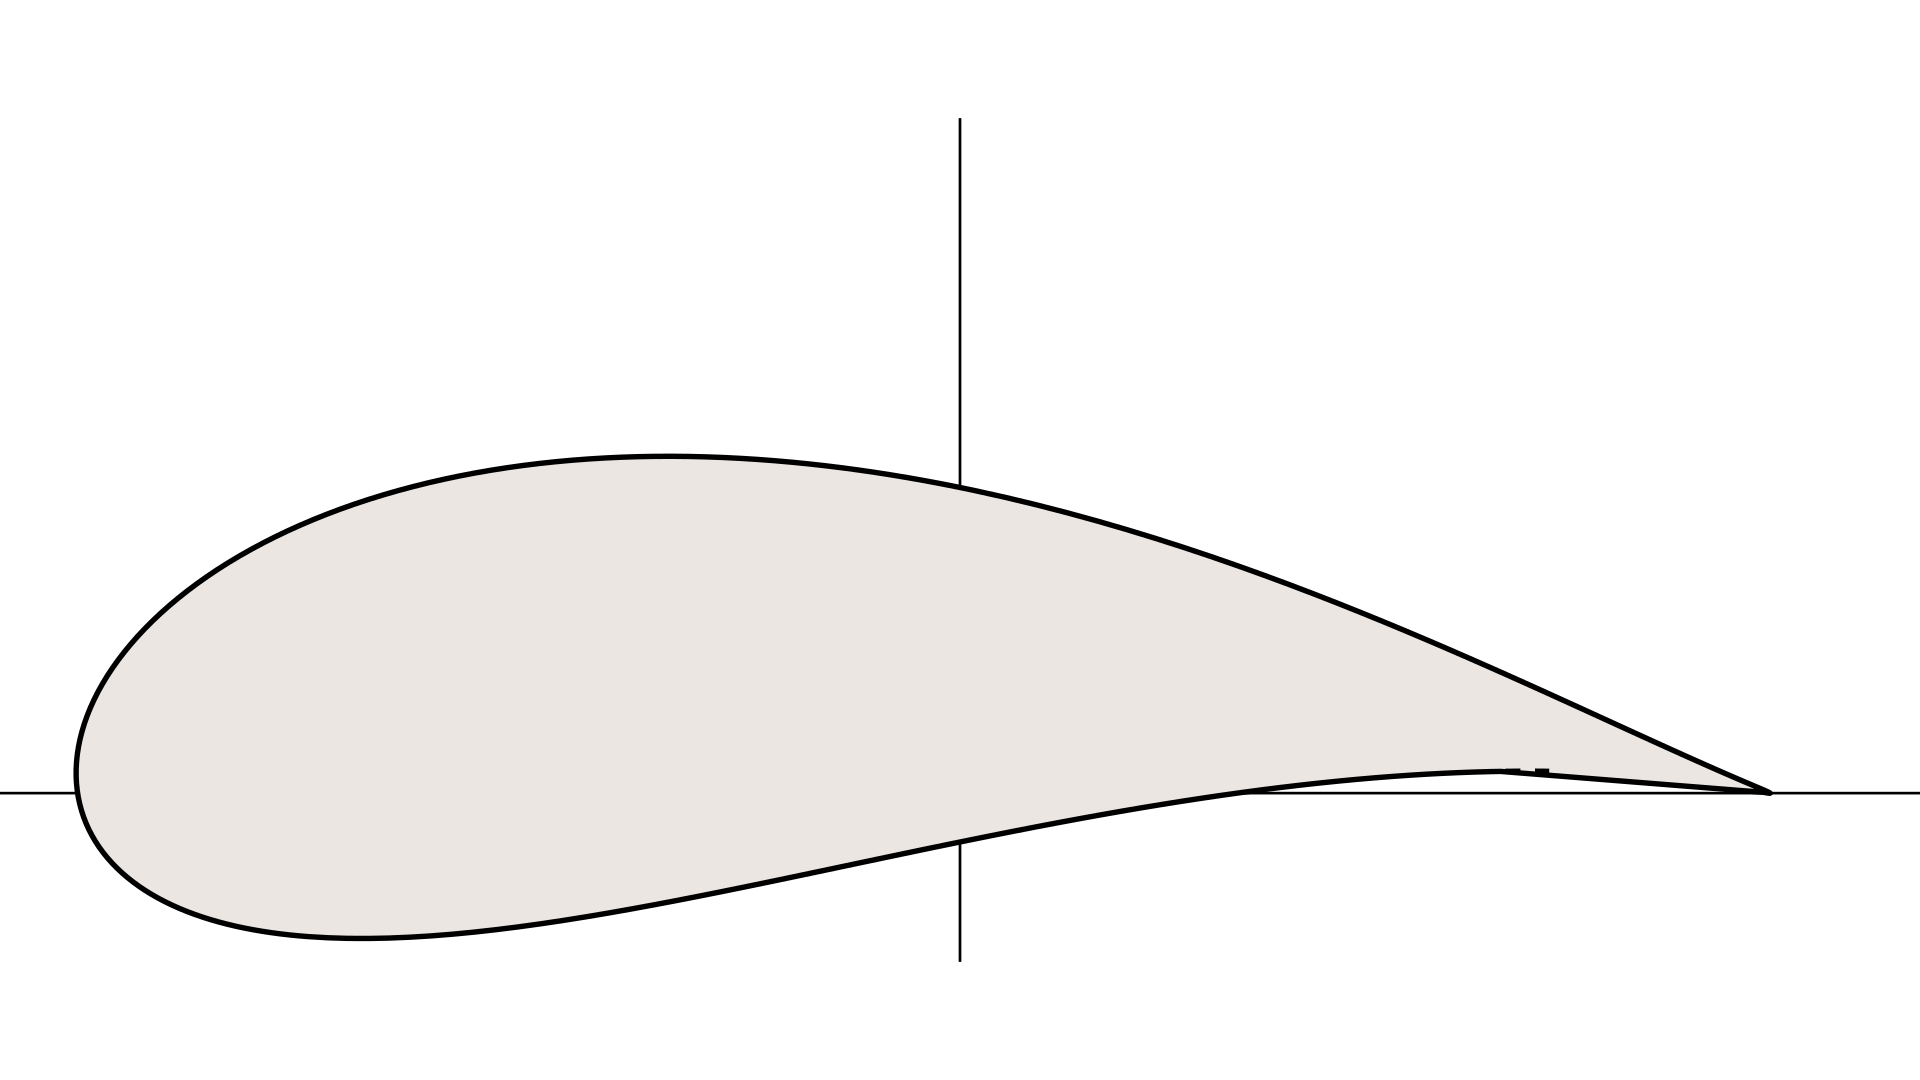
\includegraphics[width=0.95\textwidth]{Airfoil_ManimCE_v0.17.1.png}
			\end{center}
			\caption{Perfil alar de Joukowski.}
		\end{small}
	\end{figure}
	
	\noindent Este es un problema el cual parece demasiado complicado a primera vista, pero podemos valernos de uno de los resultados de flujo importantes obtenidos mediante el mapeo conforme son las soluciones del flujo de una familia de formas aerodinámicas conocidas como perfiles de Joukowski, que son el resultado de  la transformada de Joukowski, que debe su nombre a Nikolai Zhukovsky (quién la publicó en 1910), es una transformación conforme históricamente utilizada para entender algunos principios del diseño de perfiles.
	
	La transformada es
	\begin{equation}
		\zeta = \eta + \frac{a^2}{\eta},
	\end{equation}
	
	\noindent donde '$a$' es una constante que determina la fuerza y la forma de la transformación. Procedemos usando la técnica de transformación compuesta asi es como podemos pasar de un circulo a este perfil aerodinámico.
	\begin{figure}[!h]
		\begin{small}
			\begin{center}
				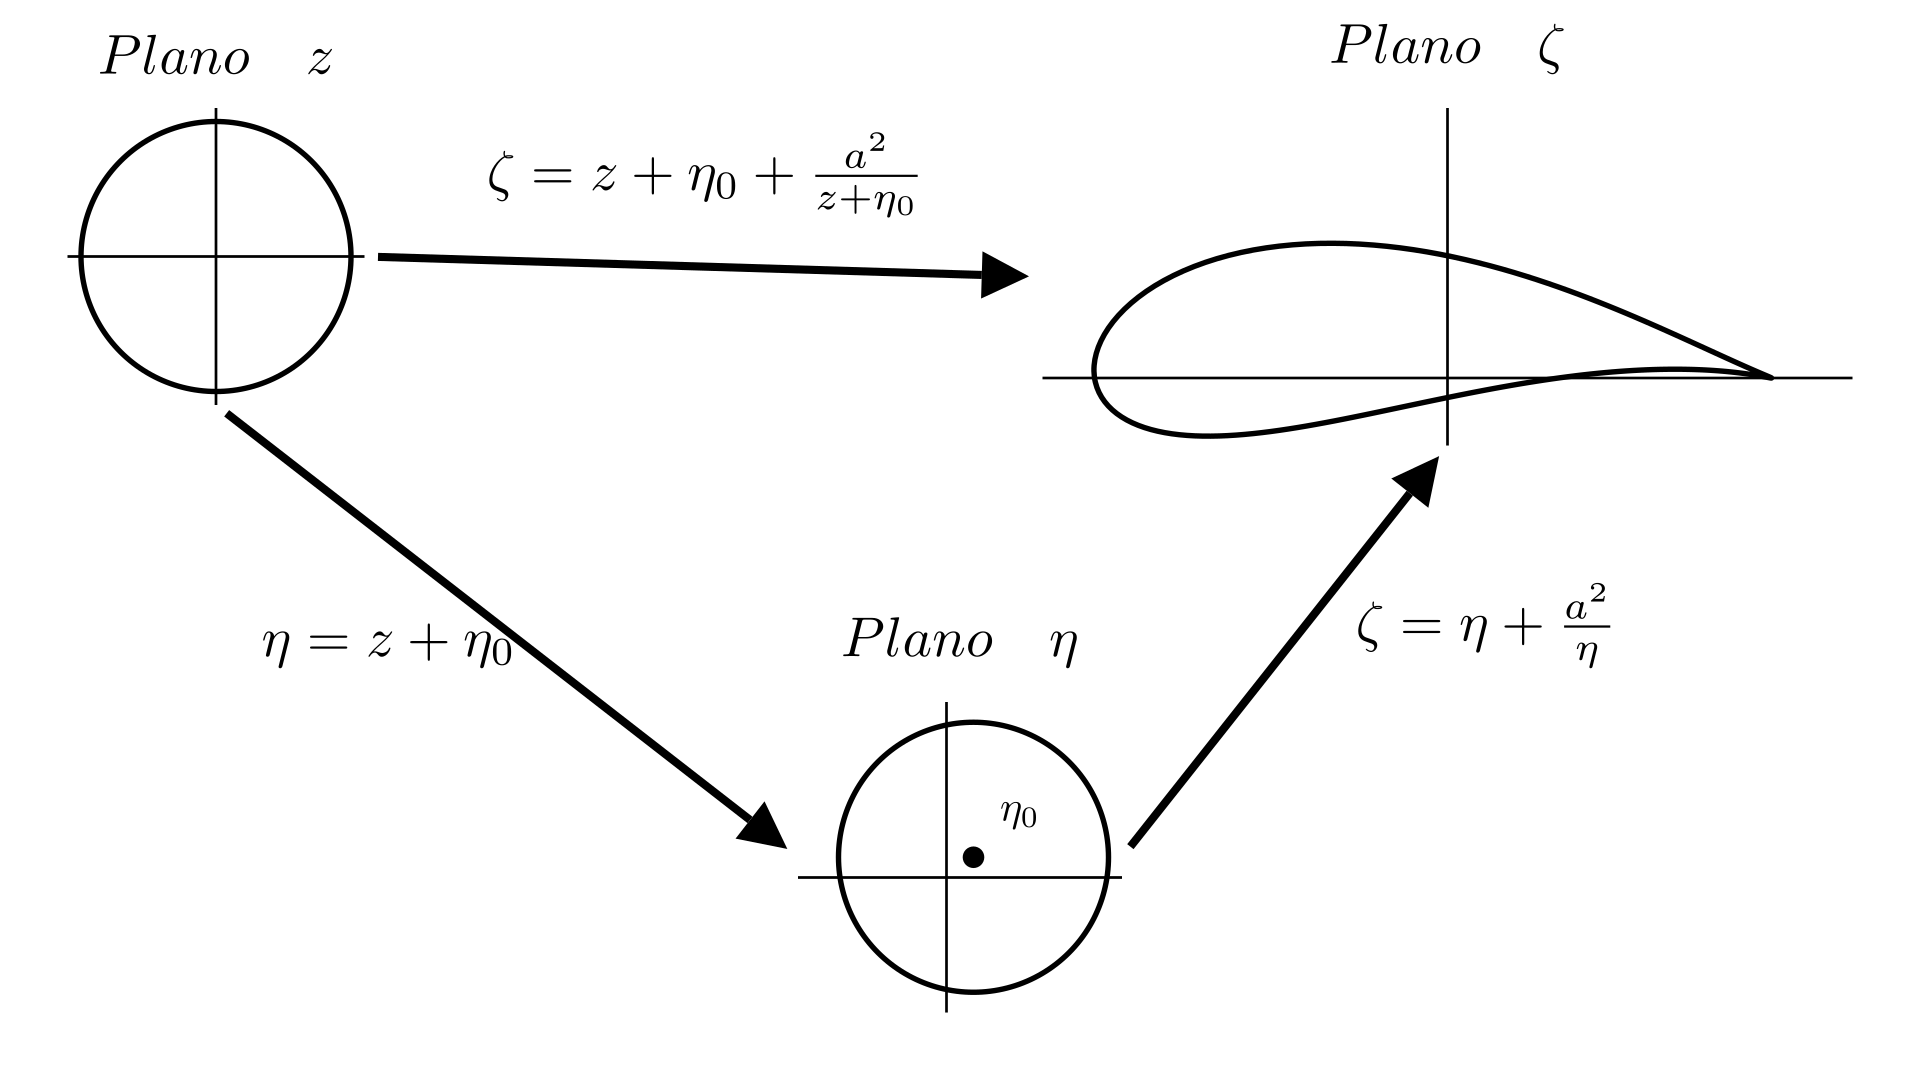
\includegraphics[width=0.95\textwidth]{JoukouskiTransform_ManimCE_v0.17.1.png}
			\end{center}
			\caption{Se muestra la transformada que se realiza para mapear un circulo unitario del plano z al perfil alar mostrado en el plano $\zeta$ mediante composición de funciones. }
			\label{TransformacionCompuesta}
		\end{small}
	\end{figure}
	
	\noindent De manera que podemos encontrar primero la solución en el flujo que pasa alrededor de  un cilindro circular con circulación para después hacer uso del mapeo conforme para transformar el cilindro en una forma aerodinámica conservando la solución.	
	
	\noindent Primero debemos de hacer unas consideraciones teniendo en cuenta la dinámica de fluidos Considere que el movimiento de un fluido esta dado por un campo vectorial de velocidades $\vec{V}(x,y,z)$, además consideremos que el fluido es irrotacional es decir que se cumple $\vec{\nabla} \times \vec{V}=0 $ lo que implica que debe de existir una función de potencial de velocidad tal que $\vec{\nabla}\varphi = \vec{V}$.Además consideremos que con la region que estamos tratando no existen fuentes ó pozos de flujo, por lo que debe de cumplirse la ecuación de continuidad para dinámica de fluidos.
	\begin{equation*}
		\frac{\partial \rho}{\partial t} + \vec{\nabla} \cdotp (\rho \vec{V}) =0		
	\end{equation*}
	Si el fluido no varia en densidad $\rho$ es decir que $\frac{\partial \rho}{\partial t} =0 $ ó $\rho = const$, implica $\vec{\nabla} \cdotp (\rho \vec{V}) = 0 \longrightarrow \vec{\nabla} \cdotp (\vec{V}) =0 $, o en términos de la función potencial
	\begin{equation}
		\vec{\nabla} \cdotp (\vec{\nabla}\varphi) = \nabla^2 \varphi =0,
	\end{equation}	 
	vemos que la función de potencial se cumple la ecuación de Laplace.
	
	\noindent La teoría de potencial	en su mayor parte es el estudio de funciones armónicas, ó en otras palabra funciones que satisfagan la ecuación de Laplace $\nabla^2u = u_{xx} + u_{yy} + u_{zz}= 0 $, en alguna region tridimensional sujeta a ciertas condiciones en la frontera de la region, si por alguna razón la función $u$ es independiente en la tercera coordenada $z$ implica que estaremos tratando con una ecuación de Laplace bidimensional $\nabla^2u = u_{xx} + u_{yy} =0$. Un resultado conocido de las funciones analíticas en variable compleja es que la parte real (ó compleja) satisface la ecuación de Laplace bidimensional en el dominio de analiticidad, siendo por esta razón que la teoría de funciones analíticas se convierte en una herramienta poderosa para el estudio de la teoría de potencial en dos dimensiones.    

	\noindent Si consideramos el flujo paralelo al plano es decir que no tendrá componentes en dirección $z$ podemos asumir que el potencial de velocidad bidimensional  $\varphi(x,y)$ tal que $\nabla^2 \varphi =0 $ en algún dominio $D$ del plano $xy$(ò también conocido como el $plano z$), y tomemos a $\varphi$ como la parte real de una función analítica compleja
	\begin{equation}
		F(z)=\varphi (x,y)	+ i \psi(x,y).
	\end{equation}
	$F(z)$ se llama el potencial complejo, donde $\psi$ es llamada  función de flujo y $\psi = c_n$, donde $c_n$ son constantes representan la lineas de flujo del fluido.
	
	%revisar 
	 %55555555555555555%%%%%%%%%%%%%%%%%%%%%%%%%%%%%%%%%%%%%%%%%%%%%%%%%%%%%%%%%%%%%%%%%%%%%%%%%%%%%%%%%%

	Si una frontera solida es colocada en en el fluido, implica que esta representa una linea de flujo, por lo que el problema se reduce  a buscar una función de flujo $\psi$ para esa frontera que pueda ser representada como $\psi=c$, y una vez que la función pueda ser encontrada la velocidad puede ser calculada con la ecuaciones de Cauchy-Riemann
	\begin{equation}
		\begin{split}
			v_x &= \frac{\partial \varphi}{\partial x} = \frac{\partial \psi}{\partial y }, \\
			v_y &= \frac{\partial \varphi}{\partial y} =- \frac{\partial \psi}{\partial x }. \\
		\end{split}
	\end{equation}
	
\section{Dinámica de fluidos}
		Si sabemos que la ecuación de Laplace cumple la propiedad de ser una ecuación diferencial lineal, eso significa que podemos añadir soluciones entre si y también sera una solución, a estas soluciones individuales se les denomina flujos elementales, que servirán como bloques de construcción para construir la solución para flujos mas complejos, existen multitud de estas funciones, pero solo nos concentraremos en aquellas que nos sirvan para este problema particular.
		\subsection{Flujo uniforme}
			El potencial complejo 
			\begin{equation}
				F(z) = U_0 e^{-i\alpha}z,
			\end{equation}
			representa un flujo uniforme con velocidad $U_0$ en la dirección del angulo $\alpha$ respecto al eje de las $x$.
			Como ejemplo vamos a calcular cual sera el campo de velocidad $\vec{V}=<v_x (x,y),v_y (x,y)>$, para eso obtendremos la función de flujo 
			\begin{equation*}
				\psi = Im[F(z)] = Im[U_0 e^{-i\alpha}z] =	U_0(y \cos{\left(\alpha \right)}- x \sin{\left(\alpha \right)} ),
			\end{equation*}
			recordando que $v_x = \frac{\partial \psi}{\partial y}$ y $ v_y = -\frac{\partial \psi}{\partial x}$, tenemos que
			
			\begin{equation*}
				\begin{split}
				v_x &= U_0 cos(\alpha),\\
				v_y &= U_0 sin(\alpha).\\
				\end{split}
			\end{equation*}
			%%%%%%%%%%%%%%%%%%%%%%%%%%%%%%%%%%%%%%%%%%%%%%%%%%%%%%%%%%%%%%%%%%%%%
			\begin{figure}[!h]
				\begin{small}
					\begin{center}
						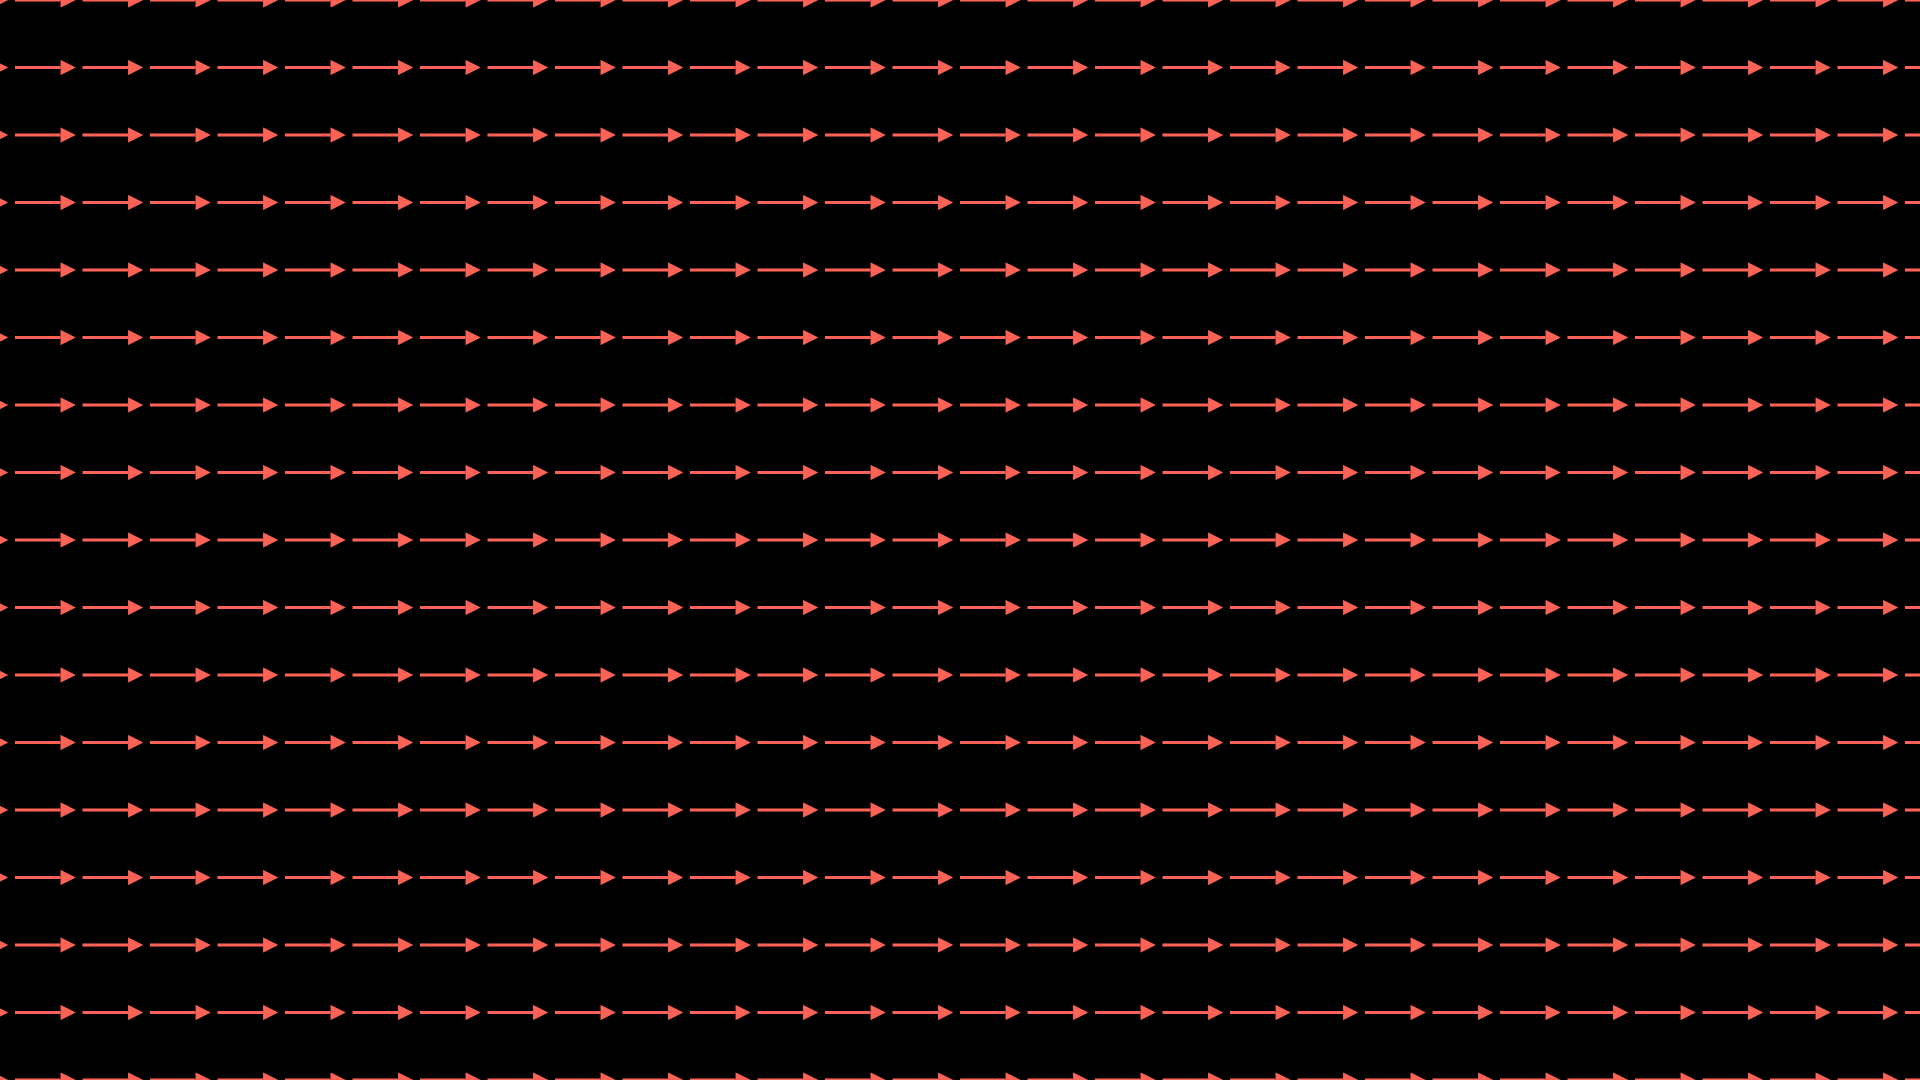
\includegraphics[width=0.95\textwidth]{uniformFlow_ManimCE_v0.17.1.png}
					\end{center}
					\caption{Campo vectorial de velocidades uniforme de magnitud $U_0 $con angulo $\alpha = 0$.}
				\end{small}
			\end{figure}
			

		\subsection{Vórtice}
			Un vórtice de magnitud $\Gamma $ en el origen esta representado por la función de potencial compleja
			\begin{equation}
				F(z)= \frac{i\Gamma}{2 \pi} Log(z),
				\label{PotencialVortice}	
			\end{equation}
			para $\Gamma>0$ la rotación es en sentido de las manecillas del reloj, y para $\Gamma<0$ es en sentido contrario.
			%%%%%%%%%%%%%%%%%%%%%%%%%%%%%%%%%%%%%%%%%%%%%%%%%%%%%%%%%%%%%%%%%%%%%
			\begin{figure}[!h]
				\begin{small}
					\begin{center}
						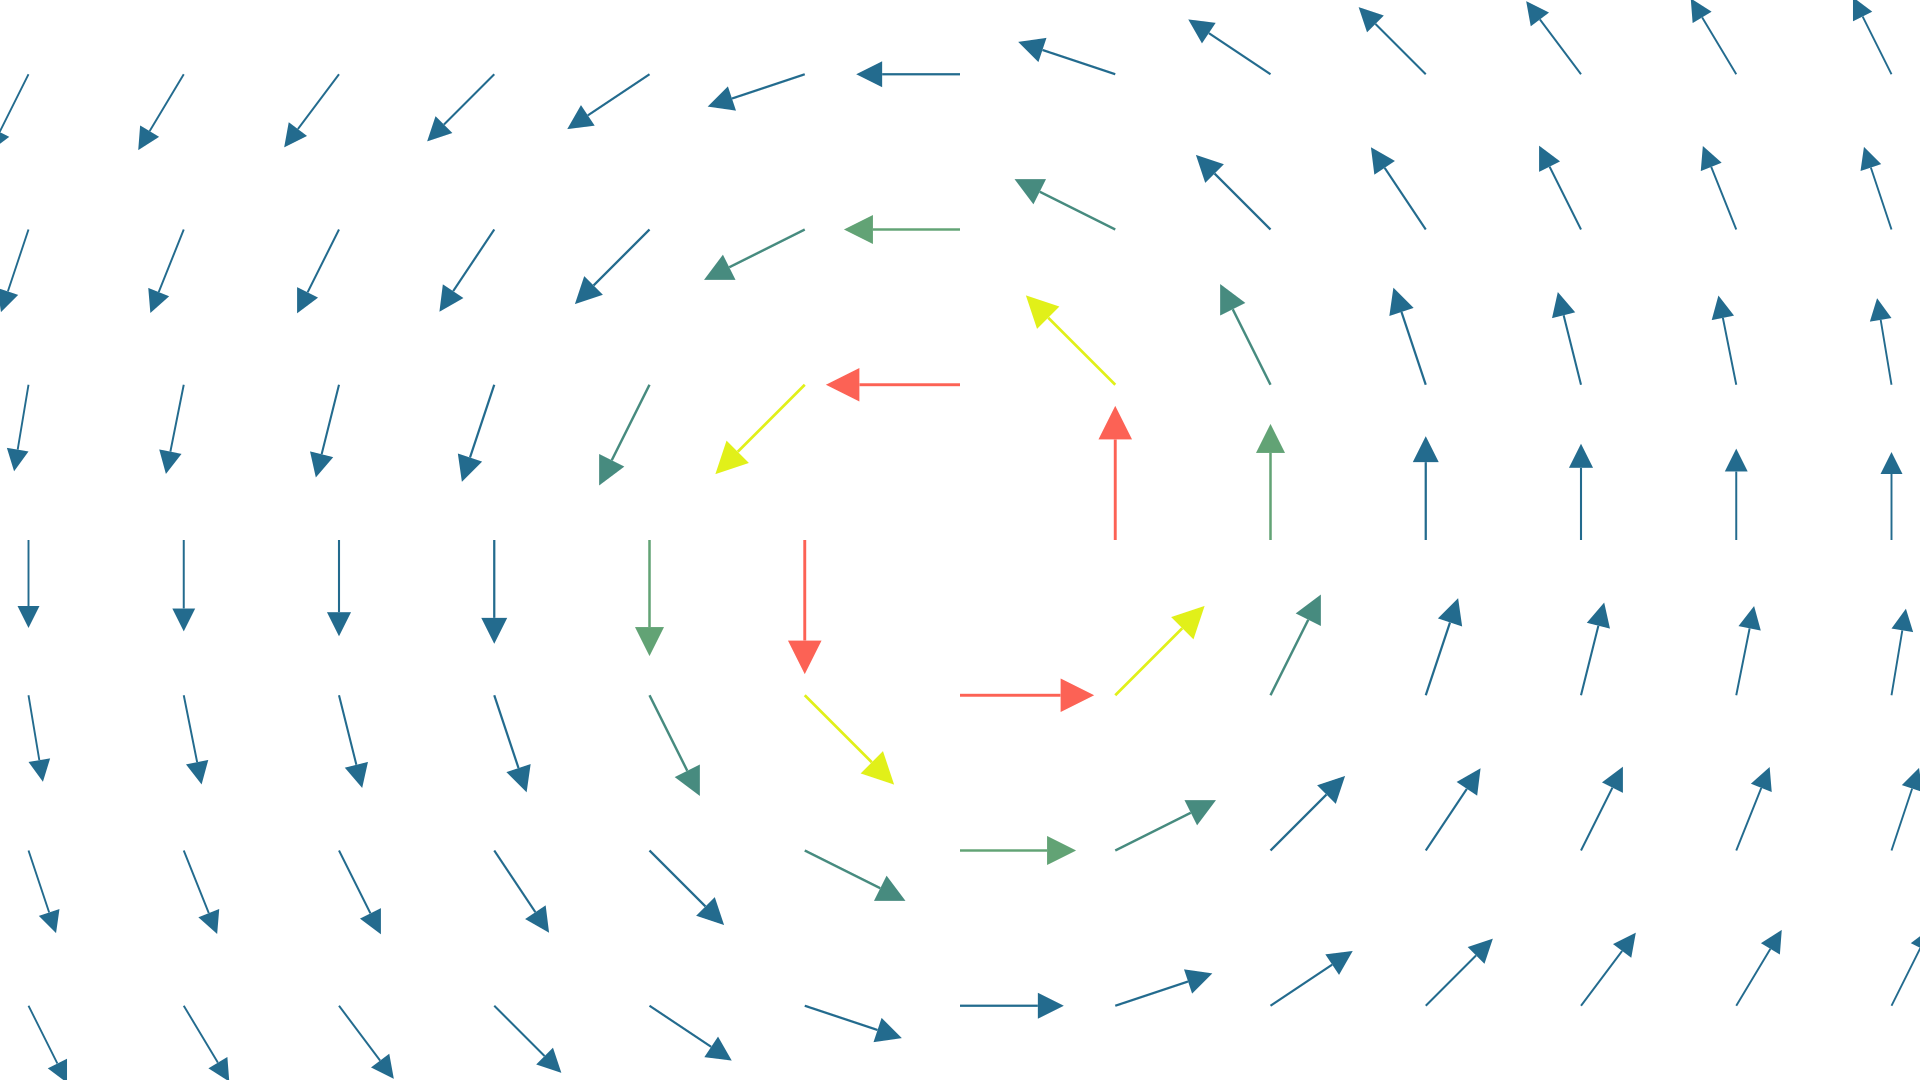
\includegraphics[width=0.95\textwidth]{vortex_ManimCE_v0.17.1.png}
					\end{center}
					\caption{Campo vectorial de velocidades de la función (\ref{PotencialVortice}).}
				\end{small}
			\end{figure}
			

		\subsection{Flujo uniforme alrededor de un circulo }
		Considere ahora un flujo uniforme con velocidad $U_0$ en la dirección $x$, con un potencial complejo $F(z)= U_0 z$, si se coloca un obstáculo circular en $|z| =R$ provocara que el fluido sea desviado.
		
		\noindent Para intentar resolver la función de potencial que tendrá el circulo usaremos un resultado encontrado por el matemático ingles L.M. Milne-Thompson.
		
		\begin{theorem}[Teorema del circulo]
			Suponga un potencial complejo $F(z)$, tal que ninguna de las singularidades de $F(z)$ ocurren en $|z|>R$, se cumple que
			\begin{equation}
				W(z) = F(z) + \overline{F \left( \frac{R^2}{\overline{z} }\right)} ,
				\label{Teorema_del_circulo}
			\end{equation}
			(Donde la barra denota el complejo conjugado) tiene las mismas singularidades que $F(z)$ en $|z|>a $, y el circulo denotado por $|z|= R $ es una linea de flujo.
		\end{theorem}
		
		\noindent Podemos darnos cuenta de que el potencial $F(z)= U_0 z$ satisface el teorema, por lo que podemos obtener el potencial complejo  del flujo al rededor de un circulo sustituyendo $F(z)= U_0 z$ en (\ref*{Teorema_del_circulo}) 

		\begin{equation}
			W(z) = U_0 z + \frac{\overline{U_0 R^2} }{\overline{z} } = U_0 z +\frac{U_0 R^2}{z} ,
			\label{PotencialCirculo}
		\end{equation}

		\noindent y la función de flujo es la parte compleja de $w$ es
		\begin{equation*}
			Im[W(z)]=\psi =  U_0 y \left( 1- \frac{R^2}{x^2 + y^2}\right).
			\label{Potencial}
		\end{equation*}
		\begin{figure}[H]
			\begin{small}
				\begin{center}
					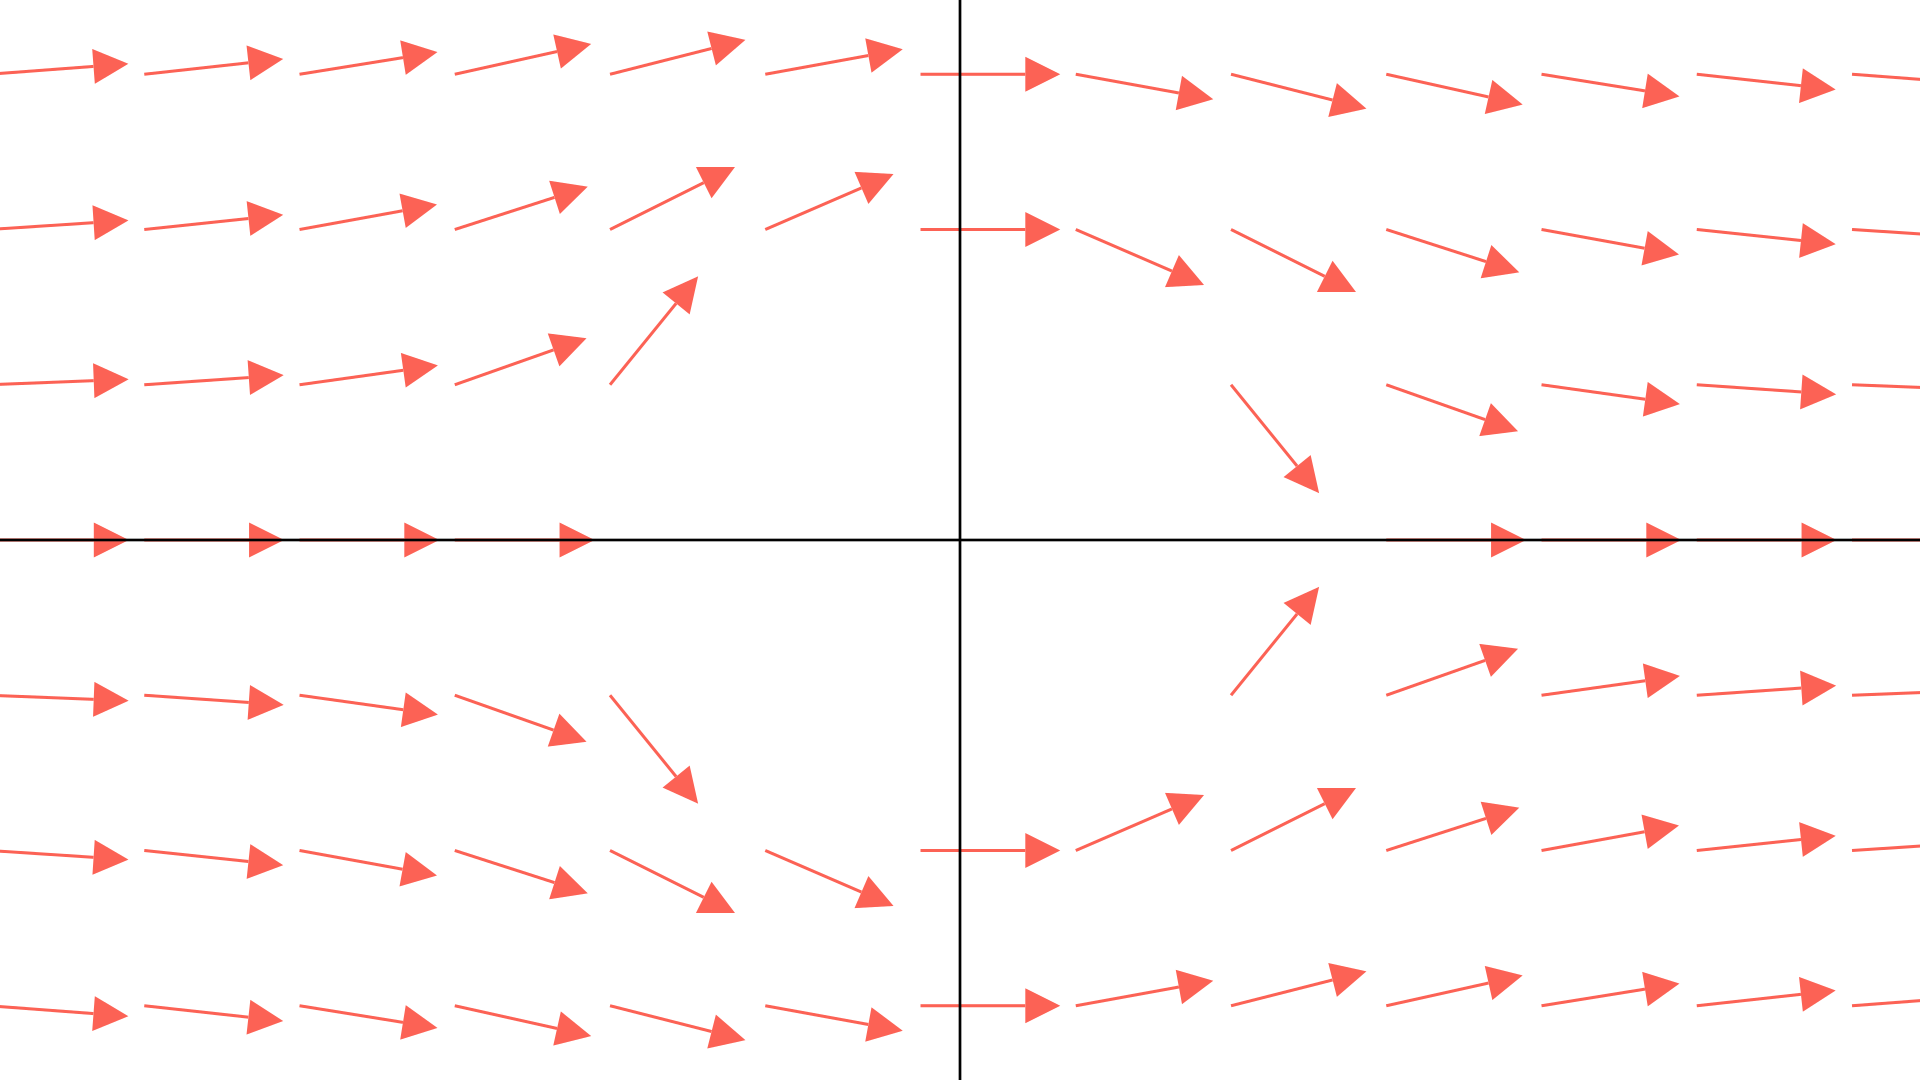
\includegraphics[width=0.95\textwidth]{FlowAroundCircle_ManimCE_v0.17.1.png}
				\end{center}
				\caption{Campo de velocidades de un fluido con un obstáculo circular.}
			\end{small}
		\end{figure}
		
		\subsection{Flujo uniforme alrededor de un circulo con circulacion}
			Si agregamos un vórtice al potencial definido en (\ref{PotencialCirculo}) se obtiene el flujo con circulación
			\begin{equation}
				W(z) = U_0z + \frac{ U_0R^2}{z} + \frac{i \Gamma}{2 \pi}\log (z),
			\end{equation}
			donde  $\Gamma$ es la circulación, hallada empleando la condición de Kutta (una condición de límite viscoso basada en la observación física utilizada con un modelo teórico no viscoso), que establece que el flujo sale suavemente del borde de salida afilado de una superficie aerodinámica, esta no sera deducida aquí por lo que solo usaremos la siguiente formula,

			\begin{equation*}
				\Gamma=4 \pi U_0 \eta_{0_y}.
			\end{equation*}
			Donde $\eta_{0_y}$ es la parte compleja del centro del circulo en el plano $\eta$ después de hacer la transformación del circulo unitario en el plano $z$ al plano $\eta$, y en este caso la función de flujo es 
			\begin{equation*}
				\psi = \frac{\Gamma \log{\left(\sqrt{x^{2} + y^{2}} \right)}}{2 \pi} - \frac{R^{2} u_{0} y}{x^{2} + y^{2}} + u_{0} y.
			\end{equation*}

			\begin{figure}[H]
				\begin{small}
					\begin{center}
						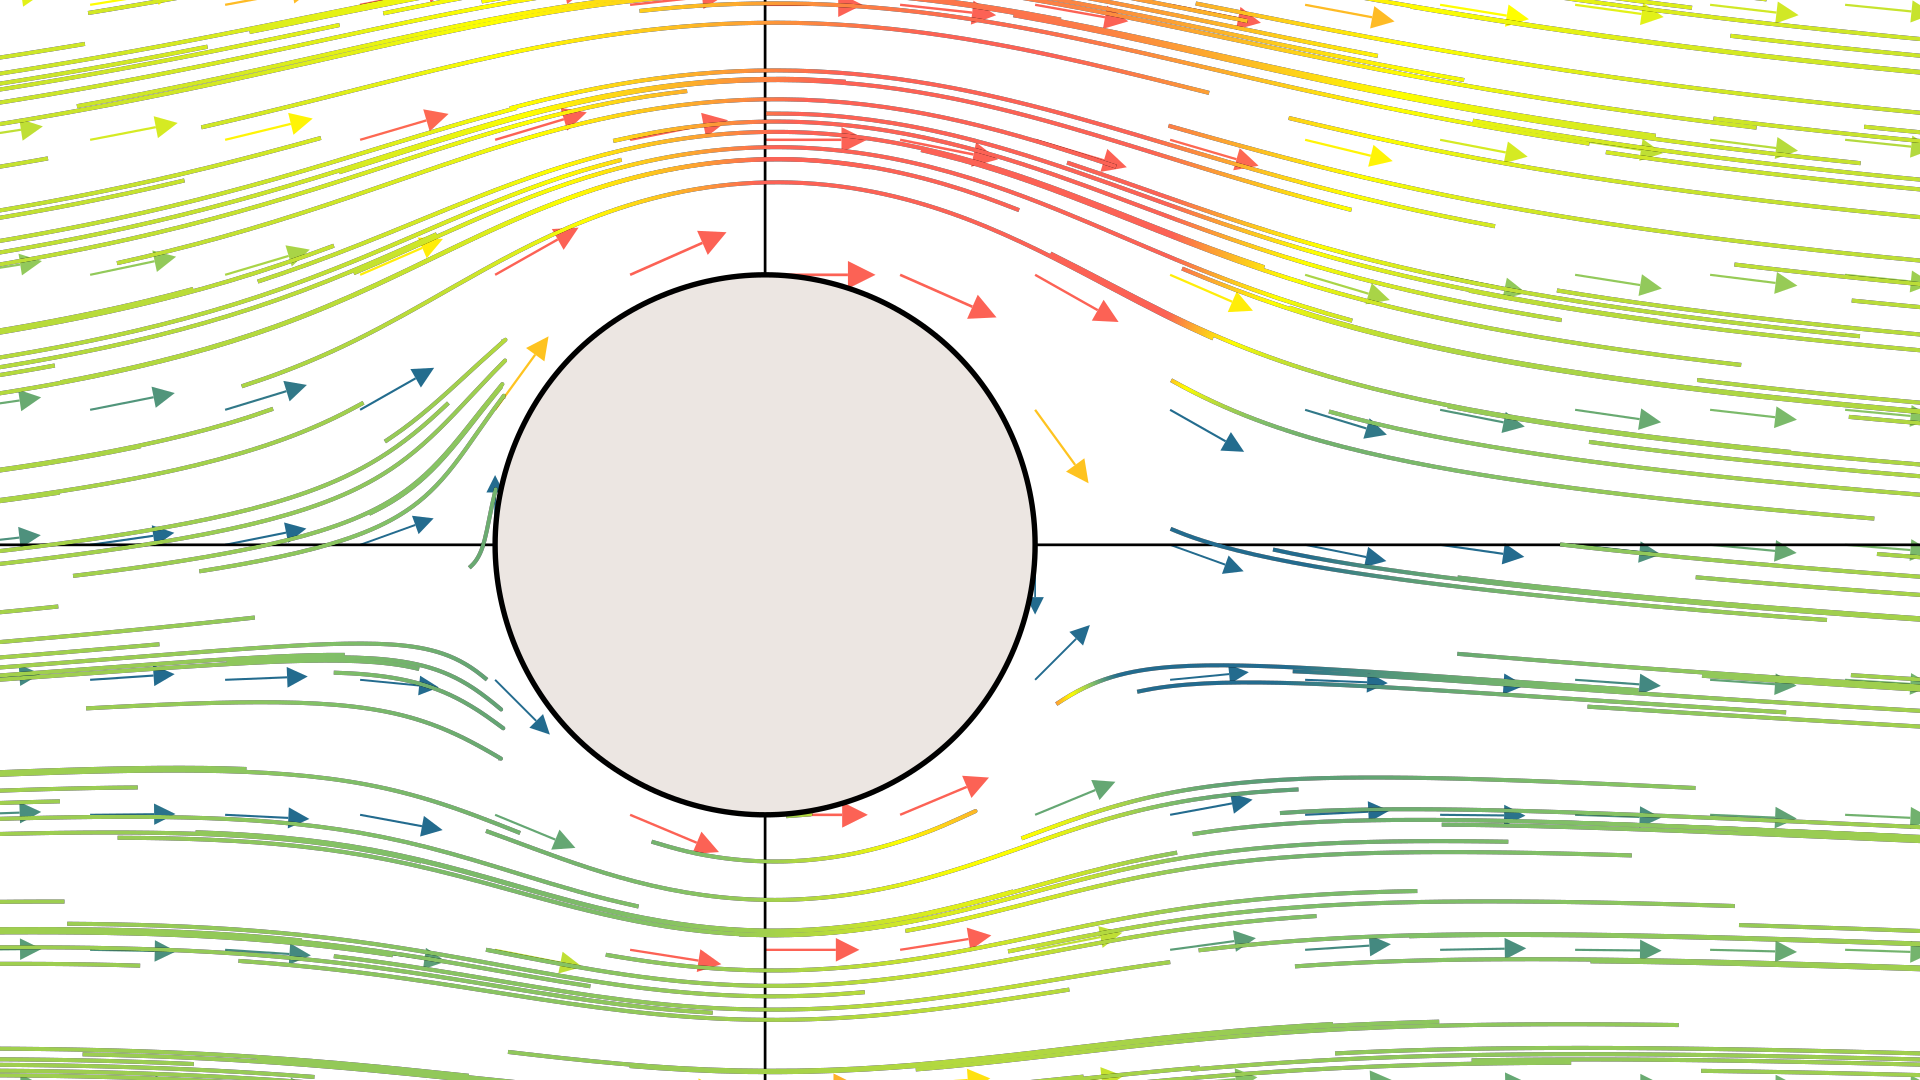
\includegraphics[width=0.95\textwidth]{StreamLinesCircleCirculation_ManimCE_v0.17.1.png}
					\end{center}
					\caption{Velocidades en un fluido con circulación (puede apreciarse como la parte superior del circulo tiene una velocidad mayor a la parte inferior de este).}
				\end{small}
			\end{figure}
			
			\subsection{Mapeo del potencial al perfil alar}
			\noindent Ahora que se conoce el potencial complejo $W(z)$ que esta asociado al $plano \: z$ es posible mapear el potencial de cada punto en el $plano \: z$ hacia hacia el $plano \: \zeta$; es decir, el potencial asociado a un punto $z_0$ sera el mismo que el potencial de un punto  $\zeta_0$ que es el resultado de evaluar $z_0$ en la transformación que hemos hecho de un circulo al perfil alar ó $\zeta_0=\zeta(z_0)$, aunque esto sea un camino valido, nuestros requerimientos nos exigen que tengamos una función de potencial complejo que llamaremos $\Xi(\zeta)$ que representa el potencial complejo en el plano $\zeta$ en función de cada punto en este mismo.
			
			\noindent Usando los desarrollos anteriores es posible encontrar cual es el potencial en un punto $\zeta_0$ encontrando cual es el potencial en el punto $z_0$ tal que $\zeta(z_0) = \zeta_0$, esto se hace mediante la inversa de la función de mapeo original.
			
			
			De manera similar a como se hizo la composición de funciones en la figura $\ref*{TransformacionCompuesta}$ se obtiene una función $Z(\zeta)$, tal que podemos evaluar en el potencial asociado al plano $z$ y obtener el potencial en el plano $\zeta$,

			\begin{equation*}
				\Xi(\zeta)= W(Z(\zeta))	= \Phi +i \Psi,			
			\end{equation*}
			y la función inversa es
			\begin{equation*}
				Z(\zeta)= \frac{1}{2}\left(\zeta \pm  \sqrt{\zeta^2 -4R^2} \right) - \eta_0 . 
			\end{equation*}
			Haciendo la evaluación $W(Z(\zeta))$ para obtener el potencial del plano $\zeta$ se obtiene
			
			\begin{equation}
				\begin{split}
					W(Z(\zeta)) = \Xi(\zeta) =& U_0 \frac{1}{2}\left(\zeta \pm  \sqrt{\zeta^2 -4R^2} \right) - \eta_0 + \frac{ U_0R^2}{\frac{1}{2}\left(\zeta \pm  \sqrt{\zeta^2 -4R^2} \right) - \eta_0}\\ 
					&+ \frac{i \Gamma}{2 \pi}\log \left(\frac{1}{2}\left(\zeta \pm  \sqrt{\zeta^2 -4R^2} \right) - \eta_0\right),\\
				\end{split}	
			\end{equation}
			cuya función de flujo $\Psi $ es
			\begin{equation*}
				\Psi=Im[\Xi(\zeta)] .
			\end{equation*}
			la cual no de derivara por cuestiones de espacio 

			(quiten esto si quieren )
			\begin{equation*}
				\Psi = \frac{\Gamma \log{\left(\left|{\eta_{0} - \frac{x}{2} - \frac{i y}{2} + \frac{\sqrt{- 4 a^{2} + x^{2} + 2 i x y - y^{2}}}{2}}\right| \right)}}{2 \pi} + \frac{R^{2} u_{0} \left(- \frac{y}{2} + \frac{\sqrt[4]{4 x^{2} y^{2} + \left(- 4 a^{2} + x^{2} - y^{2}\right)^{2}} \sin{\left(\frac{\operatorname{atan}_{2}{\left(2 x y,- 4 a^{2} + x^{2} - y^{2} \right)}}{2} \right)}}{2} + \operatorname{im}{\left(\eta_{0}\right)}\right)}{\left(\frac{x}{2} - \frac{\sqrt[4]{4 x^{2} y^{2} + \left(- 4 a^{2} + x^{2} - y^{2}\right)^{2}} \cos{\left(\frac{\operatorname{atan}_{2}{\left(2 x y,- 4 a^{2} + x^{2} - y^{2} \right)}}{2} \right)}}{2} - \operatorname{re}{\left(\eta_{0}\right)}\right)^{2} + \left(\frac{y}{2} - \frac{\sqrt[4]{4 x^{2} y^{2} + \left(- 4 a^{2} + x^{2} - y^{2}\right)^{2}} \sin{\left(\frac{\operatorname{atan}_{2}{\left(2 x y,- 4 a^{2} + x^{2} - y^{2} \right)}}{2} \right)}}{2} - \operatorname{im}{\left(\eta_{0}\right)}\right)^{2}} + u_{0} \left(\frac{y}{2} - \frac{\sqrt[4]{4 x^{2} y^{2} + \left(- 4 a^{2} + x^{2} - y^{2}\right)^{2}} \sin{\left(\frac{\operatorname{atan}_{2}{\left(2 x y,- 4 a^{2} + x^{2} - y^{2} \right)}}{2} \right)}}{2} - \operatorname{im}{\left(\eta_{0}\right)}\right)
				\label{eq:}
			\end{equation*}
			Por motivos se simplicidad no mostrare cuanto vale $v_x$ y $v_y$ pero se sobrentiende que es
			\begin{equation*}
				\begin{split}
					v_x &= \frac{\partial \Psi }{\partial y},\\
					v_y &= -\frac{\partial \Psi }{\partial x},
				\end{split}
			\end{equation*}
			y aquí la representación del flujo en el perfil alar original.
			\begin{figure}
				\begin{small}
					\begin{center}
						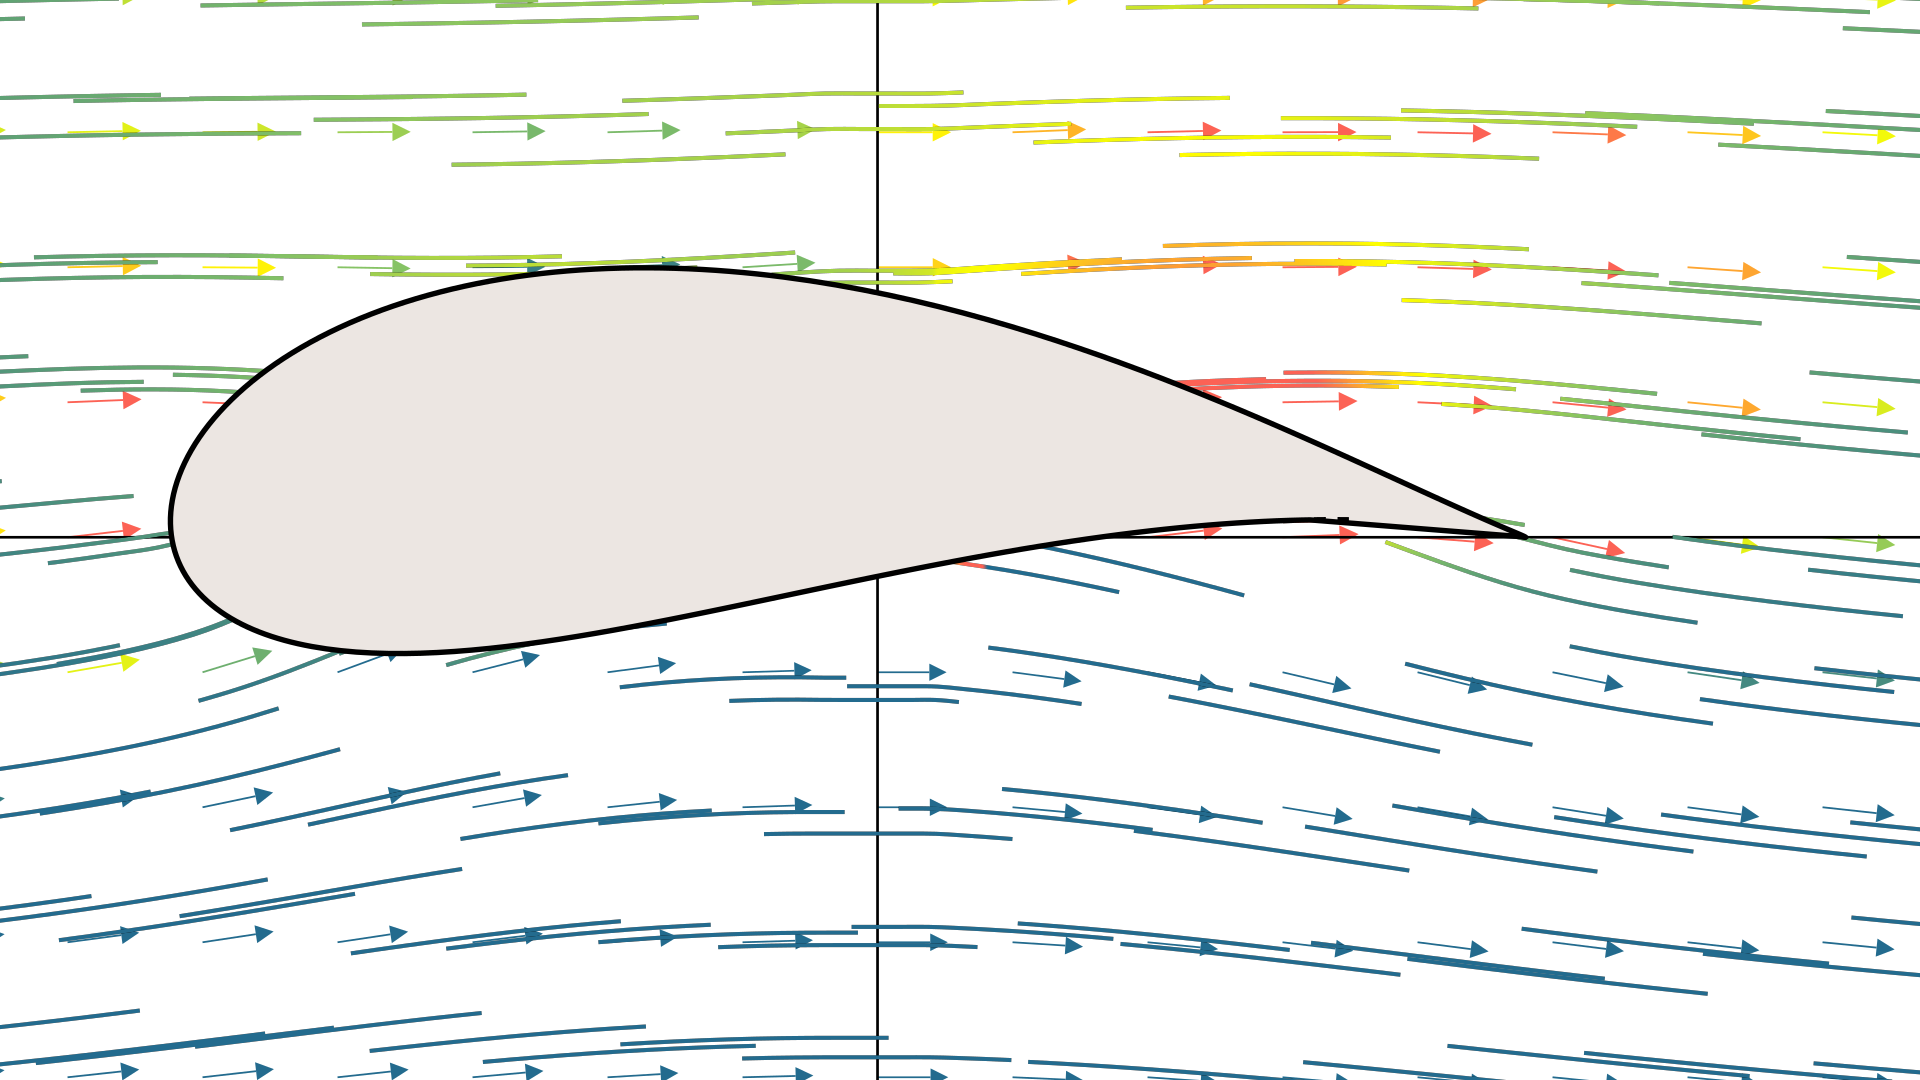
\includegraphics[width=0.95\textwidth]{StreamLinesAirfoil_ManimCE_v0.17.1}
					\end{center}
					\caption{Campo de velocidades mapeado al perfil alar original.}
				\end{small}
			\end{figure}
			
			
			
		 	
			
\newpage
\section*{Conclusiones.}

\newpage
\begin{center}
    \textbf{\Large Referencias.}
    \end{center}

\end{document}